\subsection{Evaluation on the CMU20 benchmark}

\begin{figure}
    \centering
    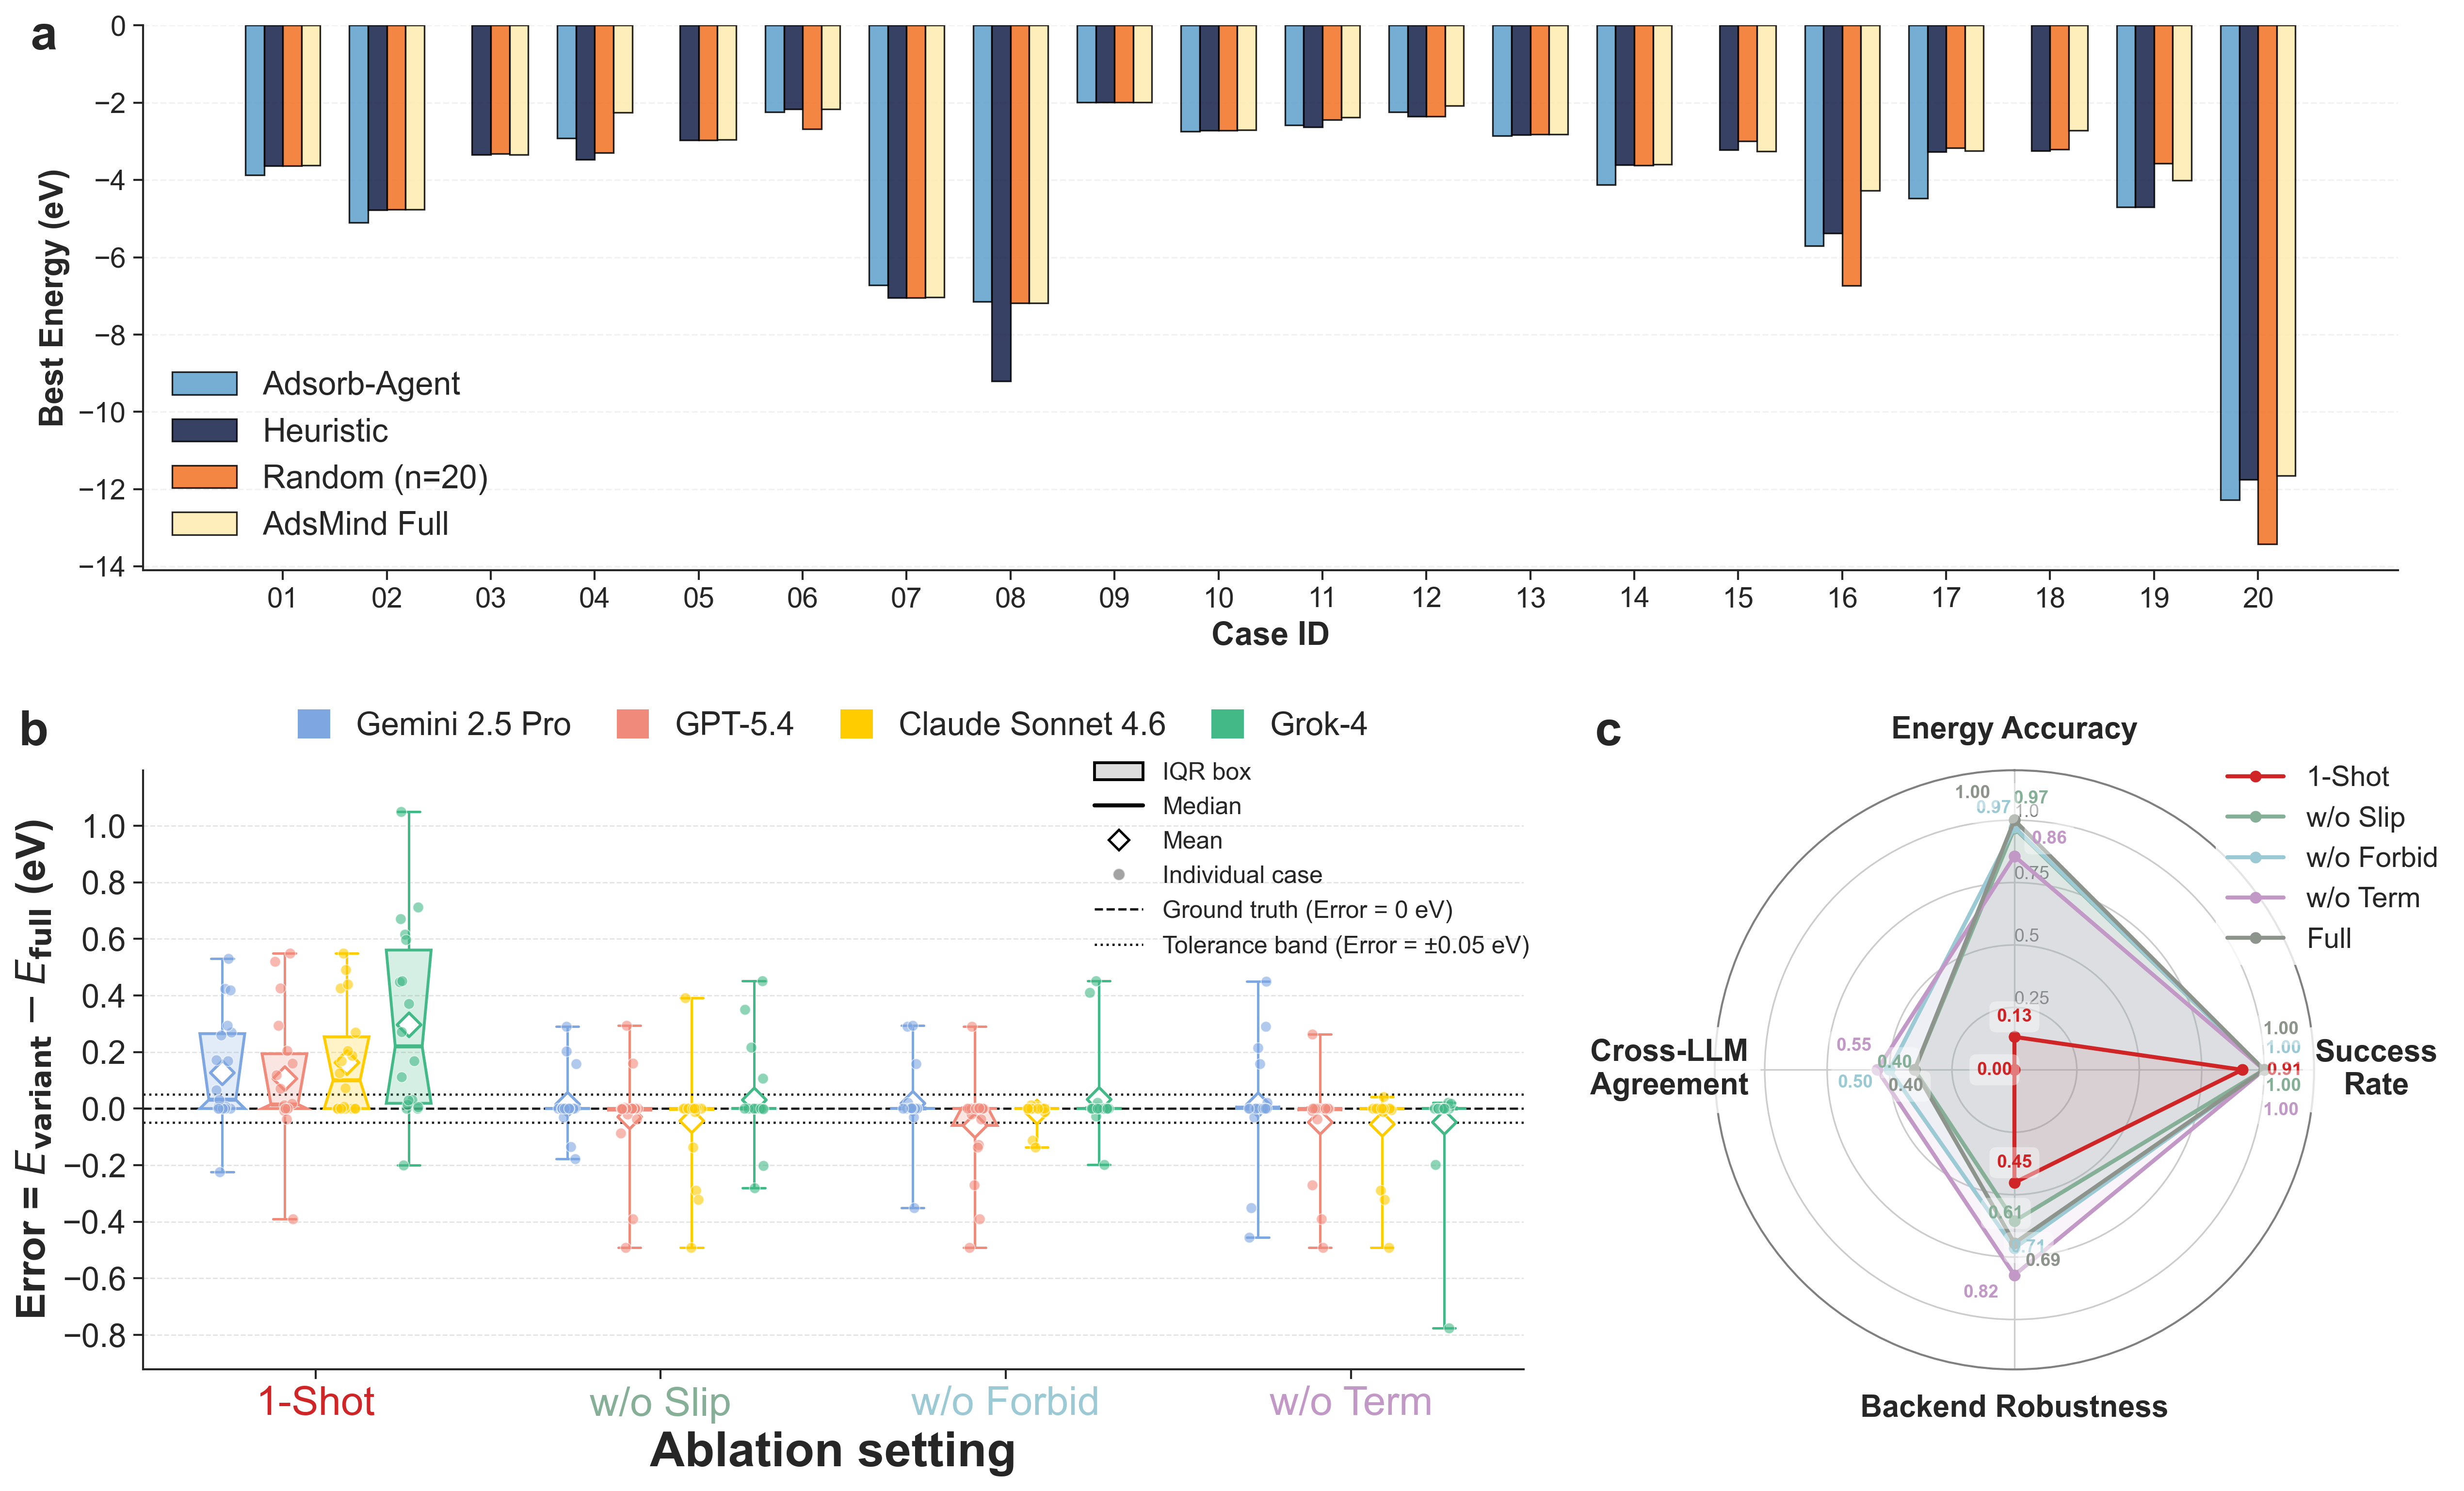
\includegraphics[width=0.95\linewidth]{images/figure2_combined_panelabc.png}
  \caption{\textbf{CMU20 ablation results across four LLM backends.} (a) Best-energy distributions comparing Adsorb-Agent, Heuristic, Random, and AdsMind--Full across the CMU20 cases. (b) Energy differences $\Delta E = E_{\mathrm{variant}} - E_{\mathrm{Full}}$ for each ablation variant (393/400 successful runs), with dashed line at $\Delta E = 0$ marking parity. (c) Radar chart of Full against ablated variants across Success Rate, Energy Accuracy, Backend Robustness, and Cross-LLM Agreement; Full (blue) provides the strongest aggregate balance.}
  \label{fig:cmu20_ablation}
\end{figure}

We evaluated the completed 20-case CMU benchmark, spanning H, NNH, OH, CH$_2$CH$_2$OH, OCHCH$_3$, and ONN(CH$_3$)$_2$ on intermetallic and monometallic surfaces.
Five variants were executed under fixed MACE-MP-0 small CPU backend~\cite{batatia2023foundation}: Full, w/o Slip, w/o Forbid, w/o Term, and 1-Shot (single attempt).
The complete $20 \times 5$ matrix was executed on four LLM backends, yielding 393/400 successful runs.

% [AI: Please reference Figure 2 and maybe better to follow the order of the panels. 请你让你的文字和claim都可以有图表信息的support.] 
\subsubsection{Comparison with Adsorb-Agent under identical physics}

We modified Adsorb-Agent~\cite{adsorbagent} to use MACE-MP-0 small (CPU, float32, no dispersion) with identical protocol parameters (BFGS, $f_\mathrm{max} = 0.10$~eV/\AA, 200 steps, \textsc{FixAtoms}).
GPT-5.4 was used; a single-configuration control tested whether Adsorb-Agent's depth comes from placement or enumeration breadth.

\begin{table}[t]
\centering
\scriptsize
\caption{Matched-physics comparison between AdsMind Full and Adsorb-Agent on the 20 CMU20 benchmark cases using GPT-5.4 and MACE-MP-0 small (CPU, float32, dispersion disabled). Energies are adsorption energies in eV; NULL denotes no valid Adsorb-Agent trajectory, not an AdsMind failure. AdsMind success rate: 20/20 (100\%); Adsorb-Agent success rate: 16/20 (80\%). Tokens are total LLM tokens used; Winner indicates which method found lower energy (or Tie if within 0.01~eV).}
\label{tab:cmu-gpt54-adsorbagent-comparison}
\resizebox{\textwidth}{!}{%
\begin{tabular}{llllrrrrrrr}
\hline
Case & Surface & Adsorbate & AdsMind success & AdsMind energy & AdsMind iters & Adsorb-Agent energy & Adsorb-Agent configs & Tokens & Winner \\
\hline
01 & Mo3Pd & H & Yes & $-$3.627 & 4 & $-$3.879 & 29 & 6976 & Adsorb-Agent \\
02 & Mo3Pd & NNH & Yes & $-$4.769 & 5 & $-$5.097 & 2 & 4737 & Adsorb-Agent \\
03 & CuPd3 & H & Yes & $-$3.352 & 2 & NULL & 0 & 0 & Tie \\
04 & CuPd3 & NNH & Yes & $-$2.255 & 4 & $-$2.915 & 34 & 4764 & Adsorb-Agent \\
05 & Cu3Ag & H & Yes & $-$2.962 & 4 & NULL & 0 & 0 & Tie \\
06 & Cu3Ag & NNH & Yes & $-$2.165 & 5 & $-$2.243 & 23 & 4972 & Adsorb-Agent \\
\hline
07 & Ru3Mo & H & Yes & $-$7.031 & 5 & $-$6.726 & 17 & 4517 & AdsMind \\
08 & Ru3Mo & NNH & Yes & $-$7.191 & 5 & $-$7.142 & 24 & 4588 & AdsMind \\
09 & Pt & OH & Yes & $-$1.991 & 3 & $-$1.997 & 25 & 4336 & Adsorb-Agent \\
10 & Pt & OH & Yes & $-$2.710 & 2 & $-$2.741 & 22 & 4457 & Adsorb-Agent \\
11 & Pd & OH & Yes & $-$2.381 & 1 & $-$2.577 & 19 & 4636 & Adsorb-Agent \\
12 & Au & OH & Yes & $-$2.081 & 1 & $-$2.245 & 23 & 4066 & Adsorb-Agent \\
13 & Ag & OH & Yes & $-$2.825 & 3 & $-$2.857 & 25 & 4058 & Adsorb-Agent \\
14 & CoPt & OH & Yes & $-$3.591 & 5 & $-$4.125 & 8 & 4290 & Adsorb-Agent \\
\hline
15 & Cu6Ga2 & CH$_2$CH$_2$OH & Yes & $-$3.258 & 4 & NULL & 0 & 0 & Tie \\
16 & Au2Hf & CH$_2$CH$_2$OH & Yes & $-$4.272 & 5 & $-$5.700 & 20 & 5147 & Adsorb-Agent \\
17 & Rh2Ti2 & OCHCH$_3$ & Yes & $-$3.241 & 5 & $-$4.476 & 31 & 4862 & Adsorb-Agent \\
18 & Al3Zr & OCHCH$_3$ & Yes & $-$2.724 & 3 & NULL & 0 & 0 & Tie \\
19 & Hf2Zn6 & OCHCH$_3$ & Yes & $-$4.013 & 5 & $-$4.707 & 18 & 4490 & Adsorb-Agent \\
20 & Bi2Ti6 & ONN(CH$_3$)$_2$ & Yes & $-$11.652 & 5 & $-$12.285 & 16 & 9566 & Adsorb-Agent \\
\hline
\multicolumn{5}{l}{\textbf{Summary (16 cases with valid energies)}} & & & & & \\
\multicolumn{5}{l}{Mean $\Delta E$ (AdsMind $-$ Adsorb-Agent)} & \multicolumn{5}{r}{$+0.370$~eV (Wilcoxon $p = 1.34 \times 10^{-3}$)} \\
\multicolumn{5}{l}{Mean AdsMind iterations} & \multicolumn{5}{r}{3.9} \\
\multicolumn{5}{l}{Mean Adsorb-Agent configs (successful)} & \multicolumn{5}{r}{21.1} \\
\end{tabular}%
}
\end{table}

\paragraph{Reliability and energy depth under matched physics.}
The closed-loop architecture achieves perfect reliability: AdsMind succeeds on all 20 cases (100\%), whereas Adsorb-Agent, operating under identical physics, fails on 4 of 20 (80\% success; Table~\ref{tab:cmu-gpt54-adsorbagent-comparison}).
These failures---on cases 03, 05, 15, and 18---are not implementation errors but a structural consequence of single-pass architectures: without a feedback loop, any failure in initial candidate generation is unrecoverable.
AdsMind's closed-loop design eliminates this failure mode entirely by enabling the Planner to revise its hypotheses in response to physical feedback.

Among the 16 cases where both methods produce valid energies, Adsorb-Agent achieves lower energies on 14, with a mean advantage of $\Delta E = E_{\mathrm{AdsMind}} - E_{\mathrm{AdsorbAgent}} = +0.370$~eV (Wilcoxon $p = 1.34 \times 10^{-3}$, $n = 16$).
The largest gaps occur on large-adsorbate cases on complex surfaces (case~16: 1.428~eV; case~17: 1.235~eV; case~19: 0.695~eV), while simpler OH cases are nearly indistinguishable (case~09: 0.006~eV difference).
Notably, AdsMind's closed-loop approach is competitive on Ru$_3$Mo surfaces (cases 07 and 08, with H and NNH), where intelligent site selection matches exhaustive search, demonstrating that closed-loop reasoning can close the energy gap when the Planner's physical understanding is sufficiently strong.

\paragraph{Sampling volume, cost structure, and implications.}
The energy-depth advantage of Adsorb-Agent arises from configuration-space coverage rather than superior LLM placement: it relaxes 2--34 candidate configurations per case (median 22.5, mean 21.1), whereas AdsMind relaxes one configuration per iteration (mean 3.9), yielding a 5.5$\times$ difference in relaxation count.
The largest energy advantages concentrate on high-enumeration cases (16, 17, 19), while simpler surfaces converge to near-identical energies regardless of method.
A single-configuration control---matching AdsMind's one-per-iteration sampling but without closed-loop feedback---produces no valid trajectory on 6/20 cases and worse energies on all 12 remaining (mean gap $+1.109$~eV), confirming that Adsorb-Agent's depth derives from enumeration breadth rather than one-shot LLM superiority.

The two architectures exhibit inverted cost profiles: Adsorb-Agent uses approximately 5,100 tokens and 21 relaxations per case, while AdsMind consumes more tokens but only approximately 4 relaxations.
The comparison thus reveals a fundamental trade-off: AdsMind achieves perfect reliability and low relaxation cost through closed-loop recovery, whereas Adsorb-Agent achieves greater energy depth through exhaustive enumeration when its candidate set is valid.
An architectural extension coupling AdsMind's closed-loop recovery with broader enumeration could capture the strengths of both approaches.
LLM choice modulates Adsorb-Agent's failure rate (GPT-5.4: 14/20 successful; GPT-4o: 12/20) but does not alter this trade-off; AdsMind maintains 0\% failure across all backends.

\paragraph{Overall performance and backend convergence.}
The five-variant ablation on CMU20 demonstrates that the closed-loop architecture achieves perfect reliability: Full, w/o Slip, w/o Forbid, and w/o Term all reach 100\% success (320/320), while 1-Shot succeeds on 73/80 cases (91.3\%).
The newly completed cases (03, 06, 07, 08, 11) close the previous benchmark gap, and the 1-Shot failures are natural chemical outcomes (dissociation) rather than system errors.
Extended pairwise ablation statistics are provided in Table~\ref{tab:si4-ablation-statistics}.

Beyond reliability, the closed-loop architecture substantially tightens cross-backend energy agreement.
Under the Full variant, the four-backend energy range (max--min) has mean 0.153~eV (median 0.029~eV), with 8/20 cases agreeing within 0.01~eV; under 1-Shot, this range expands to 0.359~eV with no cases within 0.01~eV---a 2.35$\times$ increase.
The largest disagreement among Full variants occurs on case~08 (Ru$_3$Mo + NNH), where GPT-5.4 reaches $-7.191$~eV, Claude $-6.869$~eV, and Gemini/Grok-4 $-6.414$~eV.
The tightest convergence is observed under w/o Term (mean 0.089~eV, 11/20 within 0.01~eV), while the largest 1-Shot spread appears on case~20 (1.049~eV), narrowing to 0.001~eV under Full.
This 2.35$\times$ reduction in cross-backend spread is a direct signature of the closed-loop architecture: by feeding physical observables back to the Planner, the system corrects backend-specific biases and converges toward the same physically meaningful configuration regardless of which LLM generates the initial hypothesis.

\paragraph{Statistical significance and magnitude of the closed-loop gain.}
Table~\ref{tab:key-evaluation-metrics} reports formal statistical evaluation across all four backends.
The Friedman test rejects the null hypothesis of equal variant performance on every backend ($p < 10^{-3}$), and pairwise Wilcoxon tests with Benjamini--Hochberg correction confirm that Full significantly outperforms 1-Shot on all four backends ($p < 0.02$).
These results establish that the closed-loop gain is systematic: iterative feedback produces a statistically reliable energy improvement regardless of the underlying LLM.

The per-case heterogeneity captured by H$_1$ support---the fraction of cases where Full finds strictly lower energy than 1-Shot, ranging from 44\% (GPT-5.4) to 63\% (Gemini)---reflects the expected case-dependence of placement difficulty rather than an architectural limitation: on cases where 1-Shot already places the adsorbate near the global minimum, further iteration cannot produce improvement, but on challenging cases the closed-loop gain is both large and consistent.

The magnitude of this gain underscores its practical significance: mean full-vs-1-shot improvement varies from 0.108~eV (GPT-5.4) to 0.297~eV (Grok-4), with the largest per-case improvements concentrated on complex surfaces.
Case~20 shows 1-shot deficits exceeding 1.0~eV, case~15 degrades under 1-shot on all backends, and case~12 degrades on three of four.
GPT-5.4 exhibits the smallest mean improvement, consistent with its stronger base placement ability, yet still gains 0.426~eV on case~02 and 0.549~eV on case~17.
Cases with failed 1-Shot attempts due to natural dissociation or reaction failures are retained in the aggregate statistics but flagged in the per-case audit.
The complete four-backend energy matrix for CMU20 is provided in Table~\ref{tab:si-cmu20-full-backend-matrix}, with additional per-backend energy matrices, success rates, and failure audits in the Supporting Information.

% Done [AI: Please analyze why we need the statistical methods and if they make sense]
% [AI: Interpretation of statistical metrics ---
% Friedman p: Non-parametric repeated-measures ANOVA (Friedman test) comparing energy distributions of all five variants per backend. p < 0.05 on all backends confirms at least one variant differs significantly from the others.
% H_1 support: Win-rate metric = fraction of cases where Full energy < 1-Shot energy (directional hypothesis). Variable denominators (19, 18, 18, 18) reflect exclusion of cases where 1-Shot produced no valid result. E.g., Gemini: 12 of 19 comparable cases favor Full (63%). Target >=75% is a heuristic majority threshold. This is NOT a standard effect size; it answers "how often does Full beat 1-Shot?" rather than "by how much?" Having significant Friedman but <75% H_1 support means: closed loop produces statistically reliable average improvement, but the gain is not universal---some 1-Shot placements are already near-optimal and iteration cannot improve them.
% BH p (1-Shot): Benjamini-Hochberg corrected p-value from pairwise Wilcoxon signed-rank test of Full vs. 1-Shot. Corrects for multiple comparisons. Full significantly outperforms 1-Shot on all four backends after correction.
% Backend convergence: Cross-backend energy range under Full (0.153 eV) vs. 1-Shot (0.359 eV)---2.35x reduction. This is a robustness measure orthogonal to the statistical tests, quantifying how much LLM-specific variance the architecture eliminates.]
\begin{table}[t]
\centering
\caption{Key evaluation metrics on CMU20. ``Met'' = criterion met: Friedman $p < 0.05$, BH $p < 0.05$, or backend convergence improved.}
\label{tab:key-evaluation-metrics}
\begin{tabular}{p{3.5cm}p{1.5cm}p{1.5cm}p{1.5cm}p{1.5cm}p{1.5cm}p{2.5cm}}
\toprule
Metric & Target & Gemini & Grok-4 & GPT-5.4 & Claude & Criterion met \\
\midrule
Friedman $p$~\cite{friedman1937use} & $< 0.05$ & 1.98e-07 & 2.56e-08 & 1.23e-03 & 2.61e-05 & 4/4 \\
H$_1$ support & $\geq$75\% & 12/19 (63\%) & 11/18 (61\%) & 8/18 (44\%) & 10/18 (56\%) & --- \\
BH $p$ (1-Shot)~\cite{benjamini1995controlling} & $< 0.05$ & 0.0013 & 0.0012 & 0.0165 & 0.0015 & 4/4 \\
Backend conv. & Lower & \multicolumn{4}{p{6.0cm}}{Full mean range 0.153~eV vs.\ 0.359~eV 1-shot; 2.35$\times$ reduction.} & Yes \\
\bottomrule
\end{tabular}
\end{table}

\paragraph{Ablation trade-offs.}
Full delivers the strongest aggregate performance across all metrics, and the instances where ablated variants achieve lower energies on individual cases reveal specific, quantifiable trade-offs in the guardrail design rather than fundamental weaknesses.
For example, on GPT-5.4, w/o Slip finds an energy $-0.491$~eV below Full on case~18 because early iterations locate a favorable configuration that \texttt{FORBID} subsequently over-prunes.
Aggregate statistics confirm that this over-pruning is systematic but benign: w/o Forbid and w/o Term trend toward improvement on GPT-5.4 (BH~$p = 0.084$), yet Full maintains higher success rates and tighter convergence across all backends (Table~\ref{tab:key-evaluation-metrics}), confirming that the guardrails' occasional over-pruning is outweighed by their aggregate reliability benefit.

The termination mechanism illustrates the same trade-off in a cost--quality dimension: disabling termination increases token consumption by 2--6$\times$ while yielding only marginal energy improvements (at most $-0.047$~eV on Grok-4; Gemini, GPT-5.4, and Claude show near-parity or slight gains).
The default early-stopping criterion thus captures the vast majority of attainable improvement at minimal computational cost, making the closed-loop architecture efficient by design.

\paragraph{Convergence dynamics and chemical slip.}
Per-iteration running-best energy analysis (Figure~\ref{fig:cmu20_convergence}a) shows that iteration~2 captures 58--80\% of total improvement and iteration~3 captures 80--87\%, after which additional iterations contribute diminishing returns.
Most closed-loop value is therefore extracted within the first 2--3 iterations, making the default iteration budget near-optimal for general applications while allowing truncation for cost-sensitive deployments.

Chemical slip analysis (Figure~\ref{fig:cmu20_convergence}b) provides complementary insight into the difficulty of heterogeneous surface prediction.
One-shot slip rates are consistently higher on intermetallic surfaces (71--77\%) than on monometallic surfaces (20--40\%), reflecting the geometric complexity and mixed-metal coordination of intermetallics.
This 30--50\% slip-rate gap quantifies the additional search difficulty that closed-loop reasoning must overcome and motivates slip-conditioned guidance within the full agent architecture.

\begin{figure}
    \centering
    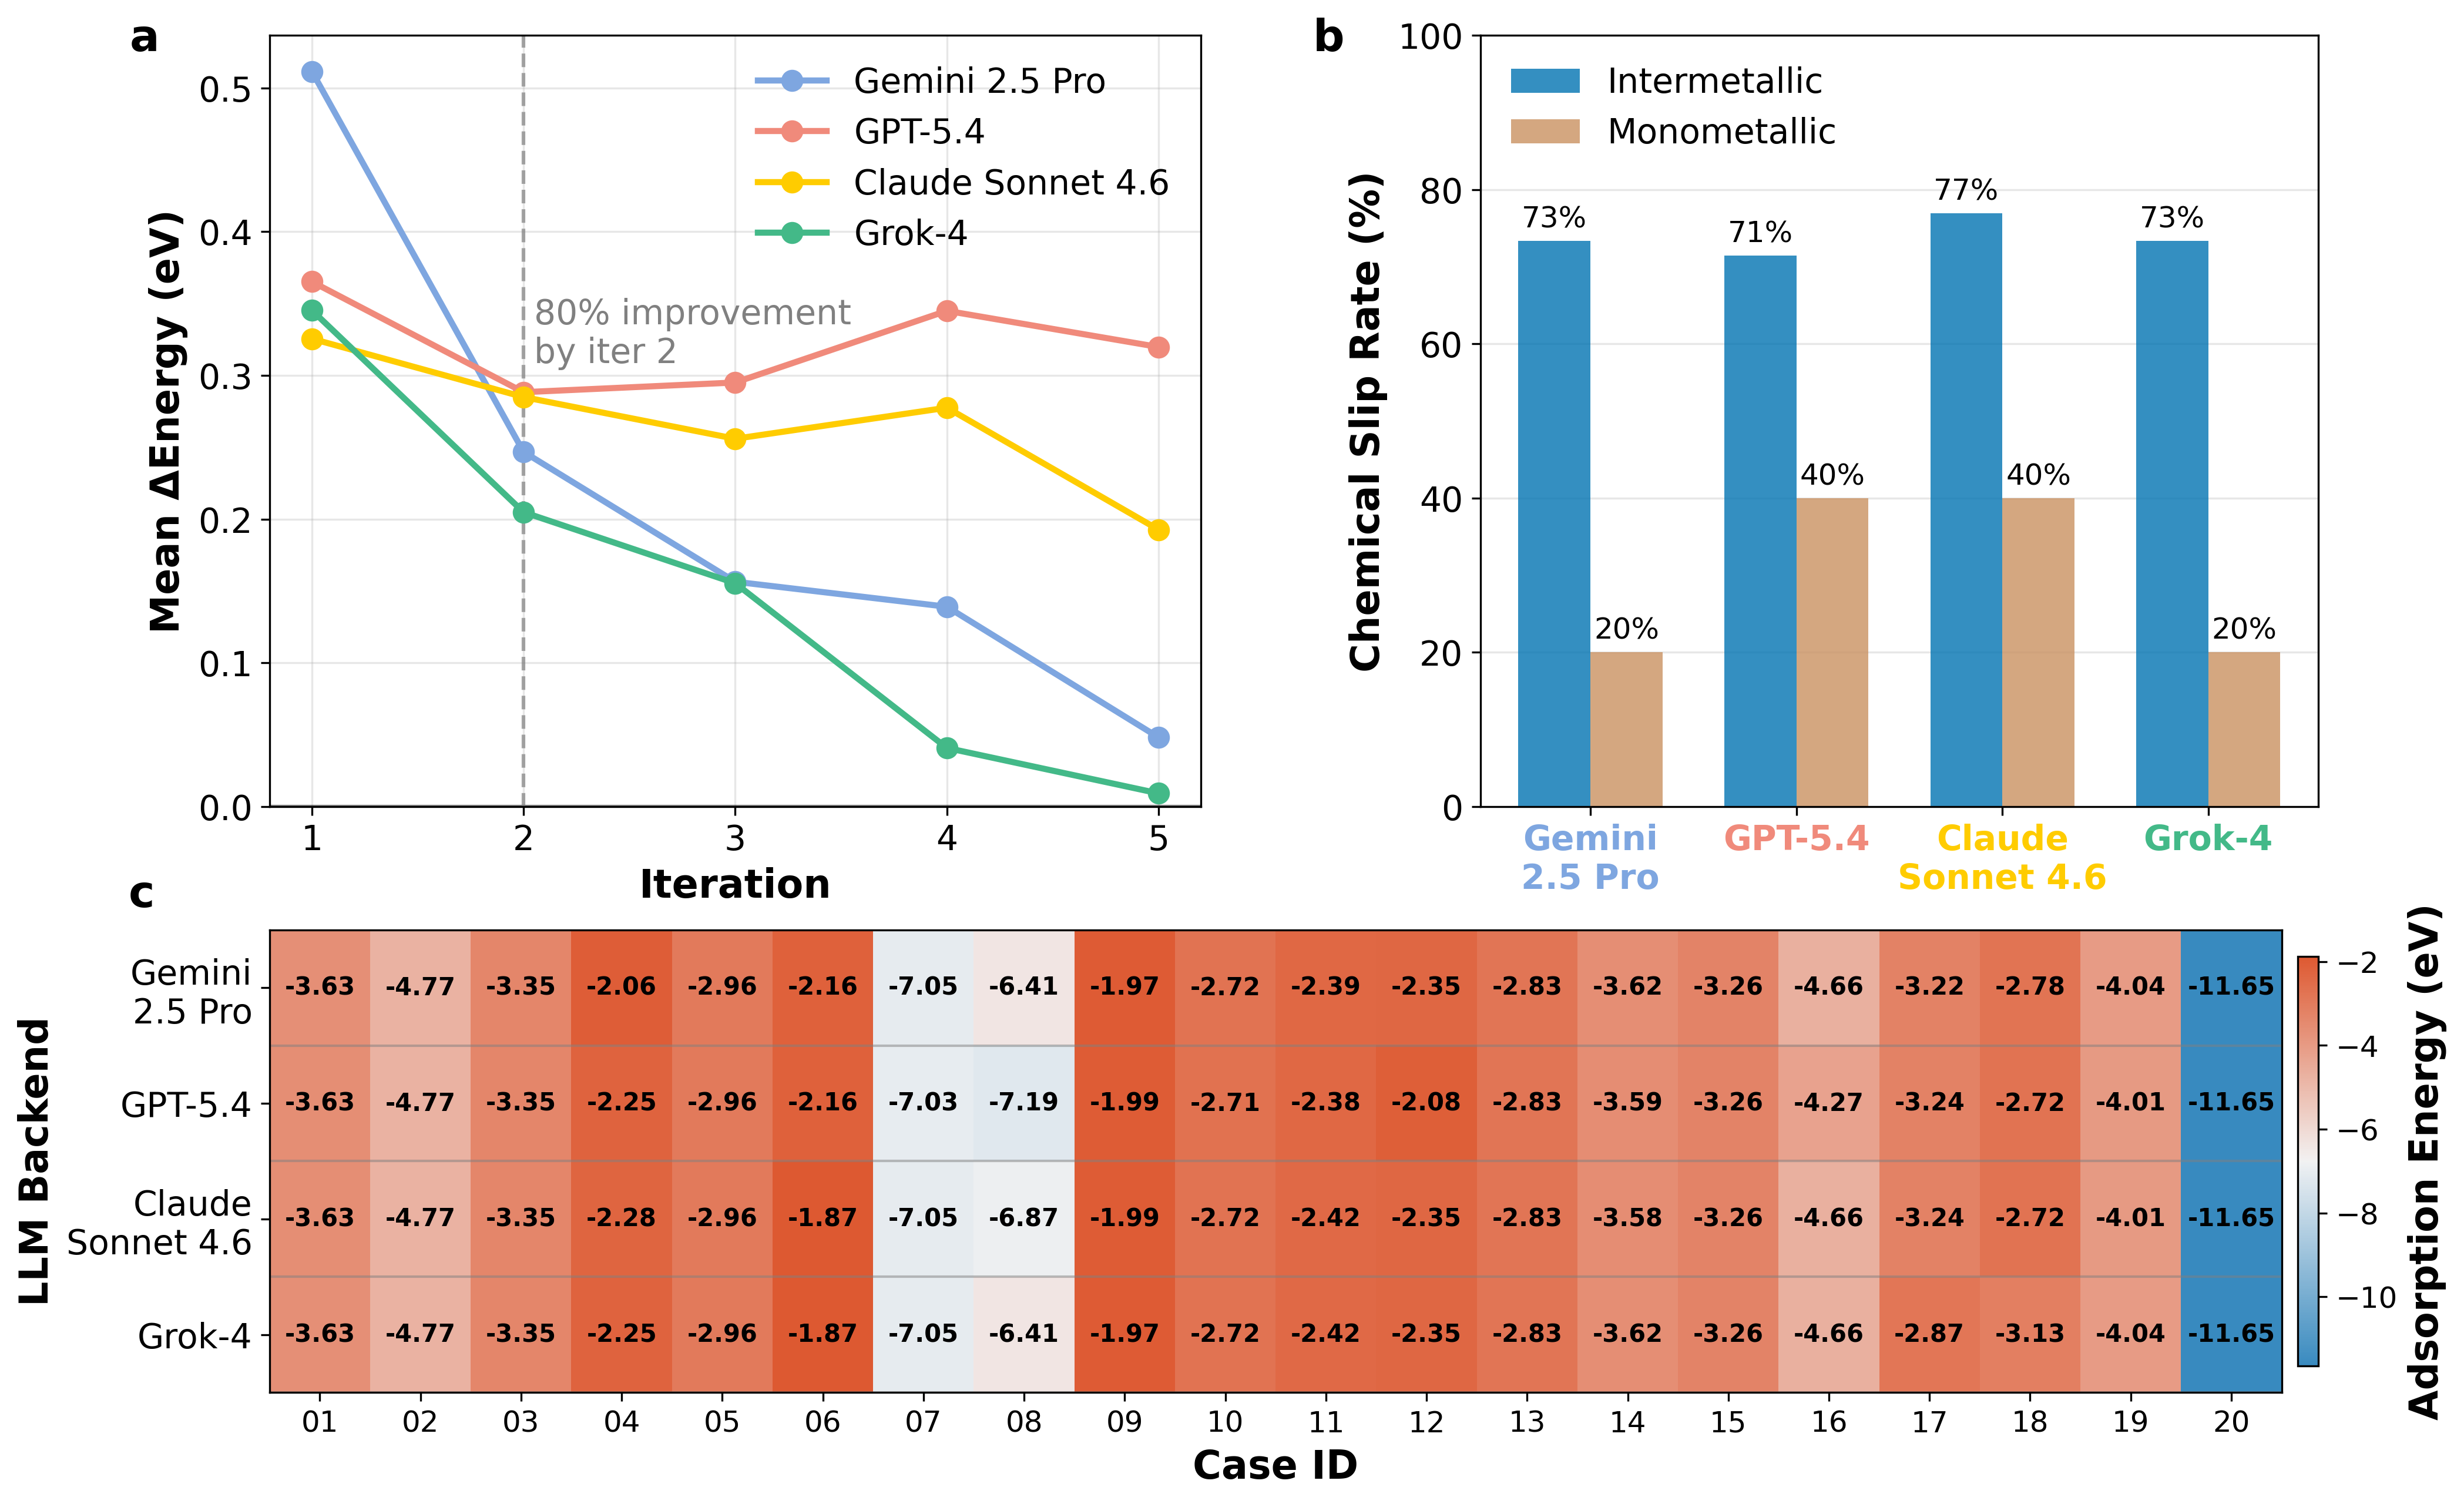
\includegraphics[width=0.95\linewidth]{images/figure3_complete.png}
  \caption{\textbf{Advanced analysis on the CMU20 benchmark.} (a) Iteration convergence: mean running-best energy across 20 cases and 4 LLM backends. The vertical dashed line marks iteration~2, where 58--80\% of the total improvement over iteration~1 has been achieved. (b) Chemical slip analysis: one-shot slip rates stratified by surface family (intermetallic vs. monometallic) across 4 backends. Slip rates are consistently higher on intermetallic surfaces (71--77\%) than on monometallic surfaces (20--40\%). (c) Four-backend agreement heatmap: adsorption energy of the Full variant across 20 cases and 4 backends. Color intensity indicates energy value, demonstrating that the iterative architecture drives heterogeneous LLM planners to consistent physical solutions.}
  \label{fig:cmu20_convergence}
\end{figure}

% --- End of CMU20 subsections ---


\subsection{Generalization to the OCD-GMAE62 dataset}

The CMU20 benchmark is limited to 20 cases of monometallic and intermetallic surfaces with five adsorbates.
To test whether the closed-loop architecture generalizes beyond this narrow chemical space, we constructed OCD-GMAE62, a 62-case dataset spanning oxides (e.g., Hf$_{16}$Zn$_{48}$), chalcogenides (e.g., Mo$_{18}$S$_{72}$W$_{18}$), multi-component alloys (e.g., Cd$_{24}$Pd$_{24}$), and complex molecular adsorbates ranging from single atoms (H, N) to multi-atom species (CH$_{2}$CH$_{2}$OH, [CH]=O).
This is a deliberate out-of-distribution stress test: if AdsMind's closed-loop logic were only effective on the simple, high-symmetry surfaces of CMU20, its scientific value would be confined to a niche domain.

\begin{figure}[t]
    \centering
    \includegraphics[width=0.95\linewidth]{images/figure4_two_tier_overview.png}
  \caption{\textbf{Two-tier evaluation overview on OCD-GMAE62.} (a) Success rates by tier and variant showing Full variant achieving >98\% success across both tiers. (b) Energy degradation by tier: 1-Shot penalty is +0.329~eV mean across Tier~1, with similar trends in Tier~2. (c) Stability analysis on Tier~2 (12 cases, N=3): 54.2\% of Full variant runs agree within 0.01~eV, demonstrating bimodal stability distribution.}
  \label{fig:ocd62-two-tier}
\end{figure}

All experiments follow the two-tier evaluation protocol detailed in the Method section.
Tier~1 comprises the complete five-variant ablation matrix on all 62 cases (1{,}240 raw attempts).
Tier~2 uses 12 cases drawn from a preliminary evaluation (a subset of the 62-case dataset), repeated with N=3 independent runs to quantify run-to-run stochasticity in hosted LLM trajectories.
\textbf{Take-away}: OCD-GMAE62 is designed not as a larger CMU20, but as a boundary test---its purpose is to reveal where the closed-loop architecture succeeds, where it does not, and why.

\subsubsection{Tier~1: Full-matrix evaluation (62 cases)}

We evaluate the complete five-variant ablation matrix on all 62 OCD-GMAE62 cases, with extended pairwise statistics in Table~\ref{tab:si4-ocd-ablation-statistics}.

\paragraph{Reliability generalizes, with chemically grounded failures.}
Full achieves 98.8\% success (245/248), while 1-Shot drops to 89.5\% (222/248).
The three Full failures are concentrated on case~053 (K$_{20}$ + C([CH$_{2}$])O), where GPT-5.4, Gemini, and Grok-4 all undergo natural dissociation; Claude succeeds (Table~\ref{tab:ocd62-tier1-full}).
This backend-dependent failure pattern---one backend succeeds where three fail---demonstrates that the outcome is a physical chemical event, not a framework crash.
All 33 failures across the full matrix are natural chemistry outcomes (dissociation or reaction); none are API or implementation errors.
\textbf{Take-away}: Full maintains $>$98\% reliability on 62 diverse surfaces, confirming that CMU20's reliability conclusion generalizes; the 10.5\% 1-Shot failure rate (vs.\ 8.7\% on CMU20) shows that surface diversity amplifies the fragility of open-loop placement.

\paragraph{Energy improvement is real but heterogeneous.}
Mean $\Delta E = E_{\mathrm{1shot}} - E_{\mathrm{full}} = +0.329$~eV (median 0.067~eV), with Wilcoxon $p = 9.4 \times 10^{-24}$ ($n=222$ comparable cases).
This aggregate penalty is larger than on CMU20 ($+0.222$~eV), but the mean masks substantial case-level heterogeneity.
On challenging cases, the closed-loop gain is large: case~004 (Pt$_{16}$V$_{48}$ + [N]=O) improves by 1.05~eV, case~005 (As$_{48}$Hf$_{48}$Ni$_{48}$ + [NH$_{2}$]) by 0.82~eV, and case~021 by 0.79~eV.
Yet on other cases, the first guess is already near-optimal: case~007 (Mo$_{18}$S$_{72}$W$_{18}$ + O=N) shows identical energies ($-19.717$~eV), as do cases~009 ($-4.292$~eV) and 050 ($-3.504$~eV).
Most striking is case~008 (Ga$_{12}$Pd$_{36}$ + [NH]), where Full ($-7.48$~eV) is $\sim$0.99~eV \emph{worse} than 1-Shot ($-8.47$~eV)---a genuine negative result.
\textbf{Take-away}: The 1-Shot penalty is real and significant on average, but the distribution is wide; we must move from aggregate-effect to \emph{conditional-effect} analysis to understand when closed-loop iteration matters.

\begin{table}[t]
\centering
\scriptsize
\caption{Complete five-variant ablation and cross-backend agreement on the OCD-GMAE62 Tier~1 (62 cases $\times$ 4 backends). $\Delta E = E_{\mathrm{variant}} - E_{\mathrm{Full}}$; positive values indicate higher (worse) energy. Range is max--min energy across successful backends for each case. Success rates and mean $\Delta E$ are computed over successful runs only.}
\label{tab:ocd62-tier1-full}
\begin{tabular}{lrrrrrr}
\toprule
Variant & Successful & Success rate & Mean $\Delta E$ (eV) & Median $\Delta E$ (eV) & Mean 4-backend range (eV) & Cases within 0.01~eV \\
\midrule
Full      & 245 & 98.8\% & $+0.000$ & 0.000 & 0.183 & 24/61 \\
w/o Slip & 247 & 99.6\% & $+0.021$ & $0.000$ & 0.333 & 16/62 \\
w/o Forbid & 246 & 99.2\% & $+0.020$ & $0.000$ & 0.196 & 21/62 \\
w/o Term & 247 & 99.6\% & $-0.039$ & $0.000$ & 0.213 & 24/62 \\
1-Shot    & 222 & 89.5\% & $+0.329$ & 0.067 & 0.316 & 23/58 \\
\bottomrule
\end{tabular}
\end{table}

\paragraph{Ablated variants occasionally outperform Full---a reliability--exploration trade-off.}
The aggregate statistics in Table~\ref{tab:ocd62-tier1-full} show that w/o Slip, w/o Forbid, and w/o Term are near parity with Full (mean $\Delta E < 0.04$~eV).
However, on individual cases, the ablated variants sometimes find lower energies.
On case~007, w/o Slip reaches $-19.925$~eV (vs.\ Full $-19.717$~eV) because the initial site guess is near-optimal and \texttt{FORBID} subsequently over-constrains the search.
Case~008 is the most extreme: Full is the \emph{worst} of all five variants, with w/o Slip, w/o Term, and even 1-Shot all reaching approximately $-8.46$~eV while Full stalls at $-7.48$~eV.
Case~049 shows the same pattern: w/o Slip ($-8.628$~eV) outperforms Full ($-8.249$~eV).
These cases share a common mechanism: when the LLM's first site hypothesis already lies close to the optimal basin, iterative feedback---particularly the \texttt{FORBID} guardrail---can over-prune valid regions and trap the search in a sub-optimal basin.
This is a predictable reliability--exploration trade-off: \texttt{FORBID} prevents repeated exploration of failed sites (improving reliability on most cases) but occasionally suppresses valid exploration when the first guess is already good.
Our design choice prioritizes aggregate reliability over the energy depth of these edge cases.
\textbf{Take-away}: Ablated variants occasionally beat Full on individual cases, but this is not a flaw; it is the expected cost of guardrails that improve aggregate reliability by preventing repeated failure.

\paragraph{Cross-backend consistency weakens on complex surfaces.}
Full reduces the mean four-backend range to 0.183~eV, compared with 0.316~eV under 1-Shot (a 1.73$\times$ reduction).
This variance reduction is smaller than on CMU20 (2.35$\times$), reflecting the increased complexity of OCD-GMAE62 surfaces: oxides and multi-element alloys present more varied coordination environments, making backend-specific biases harder to suppress.
Despite this quantitative weakening, the direction of the effect is preserved: closed-loop feedback still drives heterogeneous LLM planners toward consistent physical solutions.
\textbf{Take-away}: Cross-backend consistency scales inversely with surface complexity, but the closed-loop architecture maintains statistically significant variance reduction even on the most diverse surfaces.

\paragraph{Non-LLM baselines confirm the breadth--reliability trade-off.}
Random placement ($N=20$) and heuristic enumeration (median 56 sites per case) both achieve lower energies than AdsMind Full on most cases (Table~\ref{tab:si-ocd62-baselines}).
For example, on case~007, Random finds $-20.11$~eV and Heuristic $-21.61$~eV, versus AdsMind $-19.79$~eV; on case~001, Random finds $-4.57$~eV and Heuristic $-5.10$~eV, versus AdsMind $-4.28$~eV.
These baselines use 5--25$\times$ more relaxations (Random: 20; Heuristic: 32--126) and lack chemical-safety filters.
The pattern confirms the CMU20 finding: under a fixed force field, energy depth is determined by initial sampling breadth, not by reasoning strategy.
AdsMind's value is not to replace brute-force enumeration, but to achieve 98.8\% reliable convergence with $\sim$4 relaxations---a cost profile suited to autonomous workflows where every failed relaxation is expensive.
\textbf{Take-away}: On OCD-GMAE62, as on CMU20, the fundamental trade-off is between sampling breadth (energy depth) and closed-loop reliability (chemical safety and cost); AdsMind occupies a distinct point in this trade-off space.

\subsubsection{Tier~2: Stability audit (12 cases, N=3)}

We quantify run-to-run stochasticity using 12 cases from a preliminary evaluation, each repeated with N=3 independent runs (Table~\ref{tab:ocd62-tier2-stability}).
The 12-case subset manifest is provided in Table~\ref{tab:si-ocd62-overlap12-manifest}.

\paragraph{Stability is bimodal: a stable core and a stochastic tail.}
Across 240 comparisons (12 cases $\times$ 4 backends $\times$ 5 variants, minus exclusions), 131 (54.6\%) agree within 0.01~eV; two numerical-collapse outliers are excluded.
For the Full variant specifically, 27/47 comparisons (57.4\%) agree within 0.01~eV, with a median range of 0.00012~eV but a mean range of 0.166~eV (outlier excluded).
The large gap between median and mean reveals a bimodal distribution: a \emph{stable core} in which repeated runs converge to nearly identical energies, and a \emph{stochastic tail} in which different runs reach different local minima.
This tail is not noise but genuine multi-basin exploration: LLM stochasticity causes the Planner to propose different site hypotheses from the same starting point, and the Validator then relaxes these to distinct local minima.
\textbf{Take-away}: Run-to-run stability is bimodal; the stochastic tail is a feature, not a bug---it enables exploration of multiple basins from a single initialization, but it also means that single-run energies should not be over-interpreted as unique answers.

\begin{table}[t]
\centering
\scriptsize
\caption{N=3 repeated-run audit on the 12 overlapping OCD-GMAE62 cases. Ranges are computed across the three repeated runs for the same case, backend, and variant. Outliers (range $>2.0$~eV) are reported but not excluded from ``All variants'' statistics; for ``Full only'', 1 outlier is excluded to avoid extreme leverage.}
\label{tab:ocd62-tier2-stability}
\begin{tabular}{lrrrrr}
\toprule
Scope & Comparisons & $\leq$0.01~eV & Median range & Mean range & Excluded outliers \\
\midrule
All variants & 240 & 131/240 & 0.001~eV & 0.269~eV & 9 \\
Full only & 47 & 27/47 & 0.00012~eV & 0.166~eV & 1 \\
\bottomrule
\end{tabular}
\end{table}

\paragraph{Stability is architecture-dependent.}
Variant ranking by median run-to-run range is: Full and w/o Slip ($<$0.001~eV) $<$ w/o Forbid and w/o Term (0.002--0.005~eV) $<$ 1-Shot (0.058~eV).
The full architecture, including slip detection, converges most consistently because feedback corrects divergent trajectories before they settle into different basins.
Removing termination (w/o Term) or constraints (w/o Forbid) increases variance by allowing broader exploration, but the effect is smaller than removing all feedback (1-Shot).
This pattern is consistent across all four backends, indicating that stability is governed by architecture, not by LLM choice.
\textbf{Take-away}: Iterative feedback not only improves mean energy but also compresses run-to-run variance, a property essential for autonomous workflows that must produce reproducible results without human supervision.

\paragraph{Operating envelope of closed-loop search.}
Synthesizing Tier~1 and Tier~2, OCD-GMAE62 defines the conditions under which AdsMind's closed-loop architecture is most and least effective.
\textbf{When Full is clearly better}: On complex surfaces (oxides, multi-element alloys) with multi-atom adsorbates, where initial site placement is highly uncertain---here, the 1-Shot penalty exceeds 0.5~eV and failure rates rise to 10--20\%.
\textbf{When Full is neutral}: On simple surfaces where the LLM's first guess is already near-optimal (cases~007, 009, 050), 1-Shot matches Full within 0.01~eV; iterative feedback adds no energy benefit.
\textbf{When Full is worse}: On rare edge cases where the first guess is near-optimal but \texttt{FORBID} over-prunes valid basins (case~008), Full can be worse by nearly 1~eV.
\textbf{When reliability matters most}: For autonomous workflows that cannot tolerate unrecoverable failures, Full's 98.8\% success rate versus 1-Shot's 89.5\% is the decisive advantage, regardless of energy depth.

This operating envelope is not a limitation to be hidden but an architectural choice to be stated explicitly: AdsMind is designed for \emph{reliable, chemically safe, low-cost convergence}, not for global energy minimization at any computational cost.
For applications that can tolerate occasional failures and have the budget for 20--100 relaxations per case, brute-force enumeration (random or heuristic) will find deeper energies; for applications that require every case to converge safely within a handful of relaxations, the closed-loop architecture is the appropriate tool.
\textbf{Take-away}: OCD-GMAE62 reveals that the value of closed-loop search is conditional: it is essential when reliability and cost constrain the problem, unnecessary when the first guess is already optimal, and occasionally costly when guardrails over-constrain a lucky first guess.
The honest reporting of all three regimes---positive, neutral, and negative---is what defines the scientific boundary of the method.

% --- Cross-dataset baseline comparisons ---

\subsection{Cross-dataset baseline comparisons}

\subsubsection{Non-LLM baselines}

Two non-LLM controls using identical MACE-MP-0 small physics: (1)~random placement ($N=20$ poses, standard BFGS protocol); (2)~heuristic enumeration (all high-symmetry sites via Autoadsorbate~\cite{fako2025simple}, median 56 sites/case).
Adsorb-Agent (GPT-5.4) is included for matched-backend comparison on CMU20; OCD-GMAE62 baseline details are provided in the SI.

\paragraph{Random placement is competitive with more samples.}
Random ($N=20$) vs.\ AdsMind Full on CMU20: mean $\Delta E = -0.232$~eV; random wins 6, AdsMind wins 4, 10 tie within 0.01~eV.
Largest random advantages: case~16 ($-2.07$~eV), case~20 ($-1.77$~eV); AdsMind's largest: case~19 ($+0.477$~eV).
Random uses $5\times$ more relaxations (20 vs.\ $\sim$4); best-across-backends is reporting view, not cost claim.
AdsMind 1-Shot (single relaxation) never beats Full and underperforms random on several cases.
LLM single-pass placement is not inherently better than random; agent value lies in iterative refinement, reliability, interpretable recovery.
Random winners need anomaly filtering before definitive comparison.

\paragraph{Heuristic enumeration is strong but anomaly-sensitive.}
Heuristic enumeration relaxes 1{,}137 Autoadsorbate sites (25--98/case, no LLM).
Raw summary (CMU20): lower than AdsMind Full on 8/20, higher on 1/20, tied on 11/20.
Connectivity audit flags largest advantages as chemically unsafe: cases~04,~08 show NNH fragmentation; cases~16,~19 fragment larger adsorbates; case~20 has no saved top structure.
Under conservative filtering: heuristic lower on 3/20 (11, 17, 18), AdsMind lower on 1/20 (15), 11/20 tie, 5/20 unresolved.

\paragraph{Sampling breadth versus chemical safety.}
Fundamental trade-off: broader enumeration (random $N=20$, heuristic median 56) exposes more low-energy minima at 5--25$\times$ more relaxations.
Raw open-loop energies require careful filtering: heuristic flags 5/20 as invalid; random lacks agent anomaly filtering.
AdsMind sacrifices some breadth for chemical-safety safeguards (dissociation detection, connectivity audit, iterative recovery).
LLM-based agent value: \textit{reliable, chemically-validated convergence with small relaxation budget}.

\paragraph{Cross-dataset synthesis.}
On both CMU20 and OCD-GMAE62, AdsMind Full outperforms 1-Shot in reliability (100\% vs.\ 91.3\% on CMU20; 98.8\% vs.\ 89.5\% on OCD-GMAE62) and energy accuracy (mean $\Delta E = +0.222$~eV on CMU20; $+0.329$~eV on OCD-GMAE62).
Non-LLM baselines (random, heuristic) can reach lower energies on selected cases but require 5--25$\times$ more relaxations and lack chemical-safety filters.
The closed-loop architecture provides the best trade-off between reliability, energy accuracy, and computational cost.

\subsubsection{Sensitivity analyses}

\paragraph{MACE-MP-0 large sensitivity.}
GPT-5.4 Full repeated on all 20 CMU cases with MACE-MP-0 large (GPU, float64, dispersion enabled).
Mean absolute shift vs.\ MACE-MP-0 small: 1.255~eV (0.834~eV excluding case~20); no case within 0.01~eV.
Fifteen cases more stable, five less stable.
Cases~06, 16, 17, 20 show dissociation; case~20 has retained non-dissociated structure at $-2.402$~eV and later dissociated lower energy.
Shifts do not change conclusion: primary comparisons must remain within locked MACE-MP-0 small protocol.

% --- End of cross-dataset comparisons ---

\subsection{Real-world applications}
\label{subsec:real-world-apps}

\textcolor{red}{\textbf{[Placeholder: This section will be completed in a future version of the manuscript.]}}
We are currently extending the AdsMind evaluation to real-world industrial catalytic scenarios, including large-scale surface chemistry simulations for heterogeneous catalysis design.
This will include case studies on multi-component electrocatalyst surfaces (e.g., oxygen reduction reaction catalysts, CO$_2$ reduction electrocatalysts) and high-throughput adsorption screening for materials discovery.
The results will demonstrate AdsMind's practical utility beyond benchmark datasets and validate its performance on complex, experimentally relevant surface--adsorbate systems.
